In this case, 
    \begin{align}
        \vec{n} = \myvec{1\\0}
    \end{align}
    Thus,
    \begin{align}
        \vec{V} = \myvec{1-e^2&0\\0&1} \label{eq:chapters/11/11/3/20/V-val} \\
    \end{align}
Since
\begin{align}
\vec{c} = \vec{0}, \vec{u}=\vec{0}.
\label{eq:chapters/11/11/3/20/8}
    \end{align}
    From \eqref{eq:conic_quad_form},
    \begin{align}
        \vec{P}^\top\vec{VP} + 2\vec{u}^\top\vec{P} + f &= 0 \label{eq:chapters/11/11/3/20/ep1} \\
        \vec{Q}^\top\vec{VQ} + 2\vec{u}^\top\vec{Q} + f &= 0 \label{eq:chapters/11/11/3/20/ep2}
    \end{align}
    yielding
    \begin{align}
        16e^2 - f = 25 \label{eq:chapters/11/11/3/20/e1}
	\\
        36e^2 - f = 40 \label{eq:chapters/11/11/3/20/e2}
    \end{align}
which can be formulated as the matrix equation
    \begin{align}
        \myvec{16&-1\\36&-1}\myvec{e^2\\f} = \myvec{25\\40}
        \label{eq:chapters/11/11/3/20/mtx-eqn}
    \end{align}
    and can be solved using the augmented matrix.
    \begin{align*}
        \myvec{16&-1&25\\36&-1&40} \xleftrightarrow[]{R_1\leftarrow R_1-R_2} \myvec{-20&0&-15\\36&-1&40} \\
                 \xleftrightarrow[]{\substack{R_1\leftarrow\frac{R_1}{-5}\\R_2\leftarrow -R_2}} \myvec{4&0&3\\-36&1&-40} 
                 \xleftrightarrow[]{R_2\leftarrow R_2+9R_1}\myvec{4&0&3\\0&1&-13} \\
                 \xleftrightarrow[]{R_1\leftarrow\frac{R_1}{4}}\myvec{1&0&\frac{3}{4}\\0&1&-13}
    \end{align*}
    Thus,
    \begin{align}
        e^2 = \frac{3}{4},\ f = -13
    \end{align}
    and the equation of the conic is given by
    \begin{align}
        \vec{x}^\top\myvec{\frac{1}{4}&0\\0&1}\vec{x} - 13 = 0
    \end{align}
    See \figref{fig:chapters/11/11/3/20/ellipse}.
    \begin{figure}[H]
        \centering
        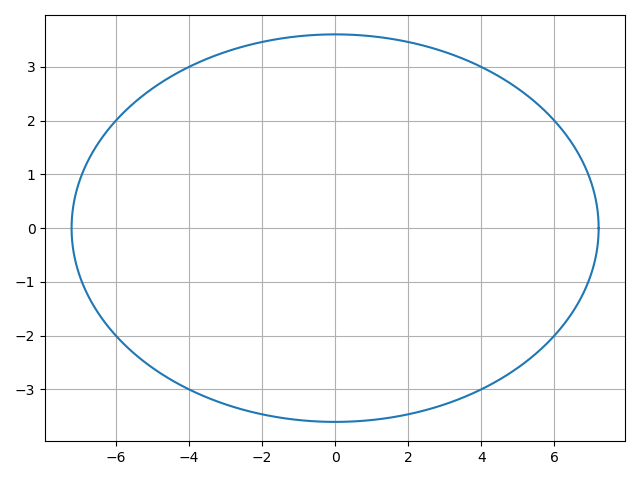
\includegraphics[width=0.75\columnwidth]{chapters/11/11/3/20/figs/ellipse.png}
        \caption{Locus of the required ellipse.}
        \label{fig:chapters/11/11/3/20/ellipse}
    \end{figure}
